\section{Evaluation}
\label{sec:eval}

We evaluate SafeDE by synthesizing the RISC-V multicore SoC into a Xilinx Kintex UltraScale KCU105 evaluation kit.

%\subsection{Simulation and verification}
\subsection{Validation}
%\subsubsection{Simulation example}
%A view extracted from the system simulation exposing the SafeDE working mechanism is found in Figure \ref{fig:chronogram}. First, at cycle 1, the chronograph shows how the lower threshold ($TH_{min}$) is crossed (instructions difference becomes smaller than 10), and the signal to stall the trail core (core2) is raised. The trail core remains stalled until the head core computes at least one instruction (just one cycle in this example). Later, at cycle 5, the upper threshold ($TH_{max}$) is crossed (instruction difference becomes larger than 15). Again, the head core (core1) is stalled until the trail core executes at least one instruction (until cycle 8 in this example).

%\subsubsection{Verification}
%To further evaluate the correct functioning of SafeDE once implemented in the FPGA, two registers that store the minimum and the maximum staggering that both cores reach during the execution are integrated. During the execution of the TACLe benchmarks set, in no case, the staggering is lower or higher than the values allowed by the thresholds.

%\begin{figure}[t!]
%\centering
%  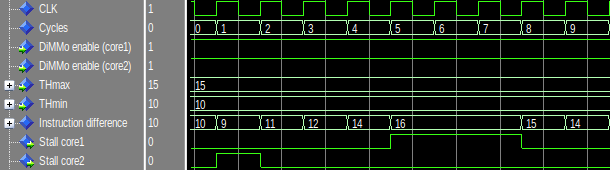
\includegraphics[width=1\columnwidth]{imgs/chronogram.png} 
%  \caption{Piece of a chronogram extracted from a simulation of the system executing the TACLe benchmark Fac and with SafeDE active forcing a controlled diversity.}
%  \label{fig:chronogram}
%\end{figure}

In order to validate the correct functioning of SafeDE once implemented in the FPGA, we have added a register recording the lowest staggering observed between the head and tail cores. We have used the TACLeBench benchmark suite~\cite{taclebench}, which is a set of open-source self-contained benchmarks intended to evaluate basic functionalities in real-time systems. They have been chosen because, since their source files already include inputs hardcoded, they can be easily compiled and run on a baremetal setup without any support to read data from files. Moreover, since some of the benchmarks are quite simple (i.e. execution times range between some hundreds and some millions of cycles), they ease debugging and validation on a simulated environment.
Therefore, we have set the staggering to 10 cycles, $TH_{stag} = 20$, and recorded the lowest staggering observed across all benchmarks. Our experiments confirm that the actual staggering has never been below this number of cycles, hence providing evidence that SafeDE works as expected.


\subsection{Execution time overhead}


%\subsubsection{Execution time overhead in a set of TACLe benchmarks}
To elucidate the impact of SafeDE in terms of computational overhead, we have run the TACLeBench benchmarks in three different scenarios:
\begin{itemize}
\item \emph{Isolation}: only one core executes the benchmark and the other core remains idle. 
\item \emph{Redundancy without diversity}: two different cores execute the same benchmark without any control mechanism. 
\item \emph{Redundancy with diversity} enforced by SafeDE: SafeDE guarantees that the minimum staggering, $TH_{stag}$, is never exceeded. 
\end{itemize}

In our evaluation, we have set $TH_{stag} = 20$ for illustration purposes. Note that the lowest value that must be used for the staggering relates to the pipeline depth of the core (7 stages in the specific platform used) given that the instructions difference is obtained using committed instructions. Hence, using a pipelined core, it could occur that, by the time staggering is about to fall below the threshold and the trail core stalled (i.e. its commit stage is stalled), the pipeline of the trail core could be executing some common instructions to those of the head core in some of the stages if the staggering is too low. Thus, we have set the threshold to be high enough so that this cannot happen in a pipeline with 7 stages and a pipeline width of 2 instructions.

%Large instruction difference between thresholds limits the overhead because it is less likely for each core to be stalled. Since this is not a limitation for most applications, we chose a conservative difference. Concretely, SafeDE is configured with $TH_{min} = 20$ and $TH_{max} = 1000$.

Note that, by using a light-lockstep approach, redundant processes are generated loading binaries twice (one for each core) in different memory segments.
%Unlike the tight lockstep approach, both cores execute different memory segments containing the same benchmark, so both executions run isolated. 
We execute each benchmark 1,000 times and use the average cycle count for each one for our evaluation to discount the effect of small variations due to, for instance, delays caused by DRAM refreshes. In any case, absolute variations observed are always in the order of few tens of cycles.

\begin{figure}[t!]
\centering
  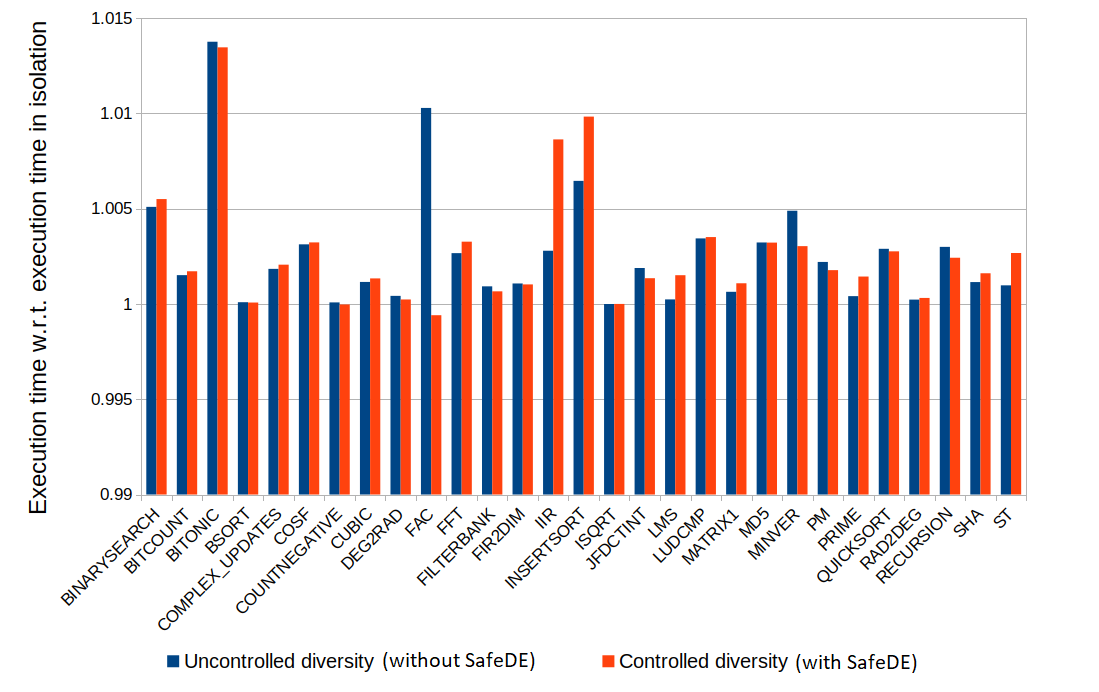
\includegraphics[width=1\columnwidth]{imgs/tacle_results.png} 
  \caption{Execution time of different TACLeBench benchmakrs normalized w.r.t. their execution time in isolation. Each benchmark is executed 1,000 times.}
  \label{fig:tacle_results}
\end{figure}

Results are shown in Figure~\ref{fig:tacle_results}. As shown, in all the cases, the execution time overhead with SafeDE w.r.t. the execution time in isolation and in two cores without SafeDE is negligible. In particular, SafeDE causes an execution time degradation in most of the cases below 0.5\%, and up to 1.3\% in one case (\texttt{BITONIC} benchmark) w.r.t. the execution time in isolation. If we compare it against the redundant execution without enforcing diversity, execution time degradation is generally below 0.1\% (in some cases performance even marginally improves), and up to 0.6\% for \texttt{IIR} benchmark.

%The biggest difference is found during the execution of the benchmark IIR and is smaller than a 0.6\%. The average overhead across all benchmarks w.r.t isolation execution is 0.17\%.

In some cases, minor performance variations between the isolation and redundant versions of the programs are observed, being those differences neither caused by interference between redundant threads, nor by SafeDE operation itself. Instead, those variations are caused by the initial core state (e.g. branch predictor state), or changes in instruction cache behavior due to changes in the memory alignment of the binaries with and without thread redundancy.
%effects related to instruction pipelining and memory alignment into instruction cache lines of the code may cause minor performance variations between the isolation and redundant versions of the programs not related to interference between redundant threads or SafeDE operation itself. 
In the case of \texttt{FAC} benchmark, since it is a small benchmark (around 700 instructions only), these tiny effects have a visible impact in relative terms (e.g. 1\% execution time increase without SafeDE and 0.1\% decrease with SafeDE). 

%As shown, in the case of \texttt{FAC} benchmark, the execution time with SafeDE is slightly lower than in isolation. Note that this behavior occurs systematically across the 1,000 runs performed for this benchmark. We have analyzed the source of this behavior in a simulated environment and found out that this benchmark is quite sensitive to the combination of pipelining effects and the state of the branch predictor. This benchmark, which is fact is a factorial program, performs frequent conditional branches. The first branches as well as the last ones may be missed. Hence, depending on how interference in the bus occurs, delays to access L2 cache (e.g. to write through data) may cause increased execution time or may avoid following mispredicted paths. This explains why uncontrolled diversity (without SafeDE) experiences interference in the bus that increases execution time, whereas controlled diversity (with SafeDE) avoids following some mispredicted paths. In any case, these are minor effects that would typically cancel out, but have an accumulative effect in our baremetal setup.

%We can see that for benchmarks Fac and Countnegative, the execution time happens to be smaller during the execution with SafeDE than in the execution in isolation. These results are explained due to a difference in the internal state of the core running in isolation and the cores running with SafeDE. This difference is caused both by synchronization mechanisms that have to be applied when two cores are active and by the SafeDE configuration previous to the execution. In these two benchmarks, this difference in the internal state affects the branch predictor behavior and causes systematically small differences in every iteration that increase the execution time in isolation w.r.t. the execution time with SafeDE. Since the overhead caused by SafeDE is minimal, the increase in the execution time due to a slower branch predictor in isolation is significant enough to end up being bigger than that overhead produced by SafeDE.

Overall, as expected, execution time increase can be regarded as negligible since the staggering threshold can be set very low (20 cycles in our evaluation), thus far below the 100$\mu$s, which correspond to many thousands of cycles, imposed by the software-only solution~\cite{SergiDFT}.


%\subsubsection{Relation between instruction difference between thresholds and execution time overhead}
%To infer how the instruction difference between both thresholds affects computational overhead, we have run the entire set of TACLe benchmarks, one after the other, 100 times and measured the total exectution time. We have done this 30 times and modifying the thresholds each time by keeping the $TH_{min}$ constant to 20 instructions, whereas $TH_{max}$ is increased. Time overhead for each pair $TH_{max}-TH_{min}$ can be seen in Figure \ref{fig:thresholds_overhead}. In the Y-axis is represented the time overhead of executing the entire TACLe benchmarks set with SafeDE w.r.t the execution time of the entire TACLe benchmarks set with only one core.

%\begin{figure}[t!]
%\centering
%  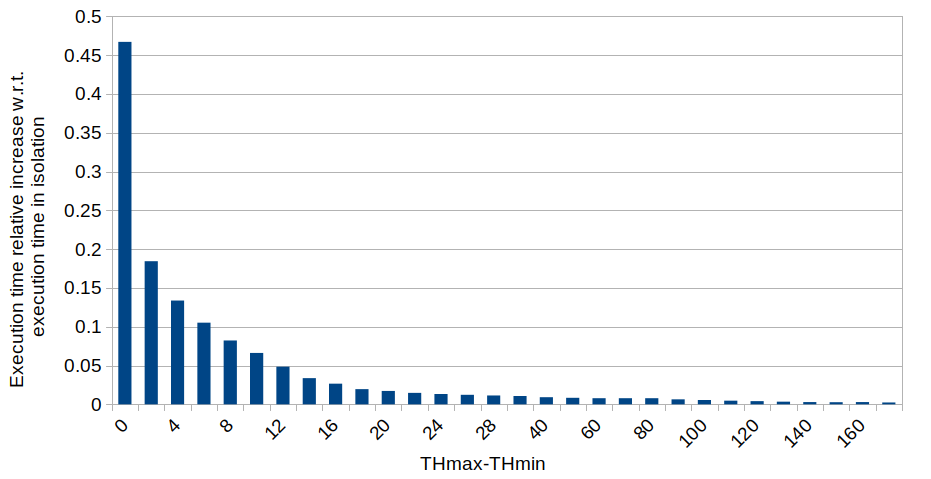
\includegraphics[width=1\columnwidth]{imgs/thresholds_overhead.png} 
%    \caption{Total execution time overhead with SafeDE of the whole set of TACLe benchmakrs w.r.t. its execution in isolation. For each run, the entire set of TACLe benchmarks are executed 100 times with the specified threshold configuration.}
%  \label{fig:thresholds_overhead}
%\end{figure}

%Overhead at low values of $TH_{max}-TH_{min}$ is above 45\%. However, overhead quickly decreases when the instruction difference between both thresholds increase. At 30 instruction distance, overhead is only 1\%, and at 170 instructions difference, overhead further reduces to 0.2\%. The more significant the difference between both thresholds, the smaller the overhead. Therefore, we can conclude that if SafeDE is used with an appropriate difference of instructions between both thresholds, the overhead becomes negligible.


\subsection{Hardware costs}

We synthesized our RISC-V design using the Vivado 2018 Toolchain and target the FPGA present in the Xilinx UltraScale KCU105. The overall cost of SafeDE implementation is 261 LUTs and 417 registers, whereas the entire SoC uses approximately 114,000 LUTs and 74,000 registers. Each core uses around 38,000 LUTs and 17,000 registers. Hence, SafeDE is a low-cost component representing just 0.23\% of the entire SoC LUTs and 0.56\% of entire SoC registers. SafeDE uses just 0.35\% of the LUTs of the pair of cores it manages, and 1.23\% of their registers. These numbers can be further improved by removing all the logic devoted to gather statistics. 

